% Sablon pentru realizarea lucrarii de licenta, conform cu recomandarile
% din ghidul de redactare:
% - https://fmi.unibuc.ro/finalizare-studii/
% - https://drive.google.com/file/d/1xj9kZZgTkcKMJkMLRuoYRgLQ1O8CX0mv/view

% Multumiri lui Gabriel Majeri, acest sablon a fost creat pe baza
% codului sursa a lucrarii sale de licenta. 
% Codul sursa: https://github.com/GabrielMajeri/bachelors-thesis
% Website: https://www.gabrielmajeri.ro/
%
% Aceast sablon este licentiat sub Creative Commons Attribution 4.0 International License.

% !TEX program = xelatex

\documentclass[12pt, a4paper]{report}

\bibliographystyle{alpha}

% Suport pentru diacritice și alte simboluri
\usepackage{fontspec}

% Suport pentru mai multe limbi
\usepackage{polyglossia}

% Setează limba textului la română
\setdefaultlanguage{romanian}
% Am nevoie de engleză pentru rezumat
\setotherlanguages{english}

% Indentează și primul paragraf al fiecărei noi secțiuni
\SetLanguageKeys{romanian}{indentfirst=true}

% Suport pentru diferite stiluri de ghilimele
\usepackage{csquotes}

\DeclareQuoteStyle{romanian}
  {\quotedblbase}
  {\textquotedblright}
  {\guillemotleft}
  {\guillemotright}

% Utilizează biblatex pentru referințe bibliografice
\usepackage[
    maxbibnames=50,
    sorting=nty
]{biblatex}

\addbibresource{bibliography.bib}

% Setează spațiere inter-linie la 1.5
\usepackage{setspace}
\onehalfspacing

% Modificarea geometriei paginii
\usepackage{geometry}
\usepackage[absolute,overlay]{textpos}

% Include funcțiile de grafică
\usepackage{graphicx}
% Încarcă imaginile din directorul `images`
\graphicspath{{./images/}}

% Listări de cod
\usepackage{listings}

% Linkuri interactive în PDF
\usepackage[
    colorlinks,
    linkcolor={black},
    menucolor={black},
    citecolor={black},
    urlcolor={blue}
]{hyperref}

% Simboluri matematice codificate Unicode
\usepackage[warnings-off={mathtools-colon,mathtools-overbracket}]{unicode-math}

% Comenzi matematice
\usepackage{amsmath}
\usepackage{mathtools}
\usepackage[table]{xcolor}
\usepackage{tabularx}
\usepackage{subcaption}
\usepackage{float}
\usepackage{interval}
\usepackage[section]{placeins}

% Formule matematice
\newcommand{\bigO}[1]{\symcal{O}\left(#1\right)}
\DeclarePairedDelimiter\abs{\lvert}{\rvert}

% Suport pentru rezumat în două limbi
% Bazat pe https://tex.stackexchange.com/a/70818
\newenvironment{abstractpage}
  {\cleardoublepage\vspace*{\fill}\thispagestyle{empty}}
  {\vfill\cleardoublepage}
\renewenvironment{abstract}[1]
  {\bigskip\selectlanguage{#1}%
   \begin{center}\bfseries\abstractname\end{center}}
  {\par\bigskip}

% Suport pentru anexe
\usepackage{appendix}

% Stiluri diferite de headere și footere
\usepackage{fancyhdr}

\usepackage{wrapfig}

% Metadate
\title{\textbf{Detectarea anomaliilor în tranzacționarea cu acțiuni}}

\author{Coman Tudor, 351 
\and Eftimie Petre-Laurențiu, 351 \and Luculescu Ștefan, 311}

\date{}

% Generează variabilele cu @
\makeatletter

\begin{document}

\maketitle
% Front matter
\cleardoublepage
\let\ps@plain

\restoregeometry
\newgeometry{
    margin=2.5cm
}

\fancypagestyle{main}{
  \fancyhf{}
  \renewcommand\headrulewidth{0pt}
  \fancyhead[C]{}
  \fancyfoot[C]{\thepage}
}

\addtocounter{page}{1}

% Rezumatul
\begin{abstractpage}

\begin{abstract}{romanian}
    
    Această lucrare explorează tehnici pentru detectarea anomaliilor în tranzacțiile bursiere și analizează impactul acestora asupra eficienței piețelor financiare. Scopul principal al studiului este identificarea și caracterizarea evenimentelor neobișnuite care pot afecta performanța activelor financiare. Pentru a valida eficacitatea metodelor propuse, se folosesc seturi de date reale provenind de pe diverse piețe financiare. Sunt prezentate atât metode din analiza semnalelor, cât şi din analiza statistică.

\end{abstract}

\end{abstractpage}

\tableofcontents

% Main matter
\cleardoublepage
\pagestyle{main}
\let\ps@plain\ps@main

\chapter{Introducere}

\section{Definiţia anomaliilor}

O \textbf{anomalie} este o entitate ce diferă semnificativ de restul enităţilor din 
setul de date. Definiţia lui Hawkins este urmatoarea\cite{hawkins1980identification}:
\textit{"O anomalie este o observaţie ce deviază atât de mult faţă de restul observaţiilor,
încât să creeze suspiciunea că a fost generată de un mecanism diferit"}.

\section{Datele folosite}

\noindent Pentru testarea modelelor, am folosit date reale de pe burs\u a, cu ajutorul bibliotecii \texttt{yfin}, ce este un Python SDK pentru API-ul oferit de Yahoo Finance. Din aceste date, am extras timestamp-ul (\^ in acest caz, trunchiat la zi) \c si pre\c tul zilnic la care s-a \^ inchis tranzac\c tionarea (``Close"), pentru a ob\c tine seria de timp. \\

\section{Indicatorul beta}

Volatilitatea ac\c tiunilor este o m\u asur\u a important\u a \^ in analiza seriilor de timp determinate de evolu\c tia pre\c turilor acestora, fiind indicatorul principal \c si un standard \^ in industrie pentru exprimarea riscului asociat cu o investi\c tie \^ in acele ac\c tiuni. Aceasta ofer\u a investitorilor \c si anali\c stilor financiari o imagine asupra incertitudinii \c si dinamicii pie\c tei. \\ 

O m\u asur\u a relativ\u a (fa\c t\u a de pia\c t\u a) pentru volatilitate este indicatorul $\beta$. Ac\c tiunile cu valori $\beta > 1$ sunt mai volatile dec\^ at S\&P 500, iar cele mai mici (dar pozitive) sunt mai pu\c tin volatile. O valoare egal\u a indic\u a o str\^ ans\u a corelare cu pia\c ta. \^ In acela\c si timp, $\beta$ poate lua \c si valori negative, caz \^ in care corela\c tia este invers\u a (de exemplu, dac\u a $\beta = -1.0$, atunci ac\c tiunea respectiv\u a are o corela\c tie invers\u a $1$ la $1$ cu pia\c ta). \cite{investopedia_beta} \\

Formula pentru calcularea indicatorului este urm\u atoarea \cite{investopedia_beta}:

$$ \beta = \frac{Cov(R_e, R_m)}{Var(R_m)}$$

unde $R_e$ - rentabilitatea ac\c tiunii, $R_m$ - rentabilitatea pie\c tii, iar $Cov$ \c si $Var$ sunt nota\c tiile uzuale pentru covarian\c ta \c si varian\c ta dintre dou\u a variabile. 

\section{Online versus offline}

Prin detec\c tia de anomalii \textbf{offline} se \^ intelege detec\c tia anomaliilor pe \^ intreaga serie de timp, iar prin detec\c tia de anomalii \textbf{online} se \^ intelege detec\c tia anomaliilor \^ in ultimul punct al seriei (cel mai recent). 

\subsection {Detec\c tia anomaliilor offline}

Prin aceast\u a abordare, se analizeaz\u a \^ intreaga serie de timp pentru a identifica modele neobi\c snuite sau schimb\u ari nea\c steptate. 

Aceast\u a metod\u a poate fi util\u a, de exemplu, \^ in cazul detect\u arii anomaliilor mai complexe, care nu reies dintr-un singur punct de date (a se vedea o anomalie de acest tip \^ in analiza f\u acut\u a mai jos pentru AAPL). \^ In plus, este o op\c tiune folosit\u a dac\u a se dore\c ste analiza datelor istorice, pentru a descoperi cum au influen\c tat anumite evenimente (crize financiare, r\u azboaie \c samd.) pie\c tele de capital. 

\subsection {Detec\c tia anomaliilor online}

\^ In general, detec\c tia anomaliilor online (\^ in ultimul punct al seriei) se face prin compararea valorii acestuia cu rezultate statistice, istorice sau date de un model predictiv. 

Un exemplu de caz \^ in care aceast\u a metod\u a ar fi aleas\u a \^ in detrimentul primeia ar fi \^ in cazul trading-ului \textit{high-frequency} (la intervale foarte scurte de timp), unde eficien\c ta computa\c tional\u a poate face diferen\c ta \^ intre o tranzac\c tie profitabil\u a sau o tranzac\c tie care genereaz\u a o pierdere. 

\subsection {Compara\c tie}

Din punct de vedere al contextului pe care \^ il de\c tine modelul, metoda offline este clar una mai bun\u a. \^ In schimb, aceast\u a metod\u a are o laten\c t\u a \^ in detectare (fiind necesar\u a analiza unei \^ intregi serii de timp), abordarea online fiind una mai bun\u a dac\u a se dore\c ste eficien\c t\u a computa\c tional\u a.
\chapter{Metode statistice}

\section{Eliminarea trendului}
\subsection{Metoda regresiei polinomiale}

\noindent Metoda constă în presupunerea că trendul seriei este un polinom de grad mic (2, 3, 4, 5) și calcularea polinomului de regresie. Pașii metodei sunt:\\

\noindent 1) Se consideră valorile seriei de timp $v = [v_0, v_1, ..., v_{n-1}]^T$ și momentele de timp $t = [t_0, t_1, ..., t_{n-1}]^T$ 
la care au fost înregistrate valorile $v$. \\

\noindent 2) Se determină trendul seriei sub forma unui polinom $P$ de grad mic $d$ $\in$ \{2, 3, 4, 5\} prin rezolvarea sistemului liniar $P(t_i)=v_i, 
i \in \{0, 1, ..., n-1\}$ în sensul celor mai mici pătrate. \\ \\
\noindent 3) Seria fără trend este $r = [r_0, r_1, ..., r_{n-1}]^T$, $r_i = v_i - P(t_i)$.\\
\\

\subsection{Metoda regresiei polinomiale - rezolvarea sistemului}
\noindent 1) Polinomul $P$ este reprezentat prin vectorul de coeficienți $c = [c_0, c_1, ..., c_d]^T$, $P = c_0 + c_1X + ... + c_dX^d$.\\

\noindent 2) Matricea sistemului este $A \in M_{n,d+1}(\mathbb{R})$, $A_{i,j} = t_i^j$, $i \in \{0, 1, ..., n-1\}$, $j \in \{0, 1, ..., d\}$.\\

\noindent 3) În ipoteza $n-1$ > $d$ (seria de timp este lungă, iar gradul polinomului este mic), matricea $A$ are rang $d+1$ și sistemul $Ac = v$ admite soluție unică în sensul celor mai mici pătrate ($c$ minimizează norma vectorului $v-Ab$, unde $b$ este un vector din $\mathbb{R}^{d+1}$).\\

\noindent 4) $c = (A^TA)^{-1}A^Tv$.

\section{Detectarea anomaliilor}

\subsection{Metoda z-score}
\noindent Ideea metodei constă în presupunerea că valorile din seria fără trend reprezintă eșantioane dintr-o distributie normală de medie $m$ 
și deviație standard $sd$. Apoi se calculează estimatorii de verosimilitate maximă \cite{normal_mle}, în acest caz media empirică pentru medie 
și varianța empirică pentru pătratul deviației standard. Pașii metodei sunt:\\

\noindent 1) Se lucrează pe serii fără trend $r = [r_0, r_1, ..., r_{n-1}]^T$.\\

\noindent 2) Se calculează media $m = \frac{1}{n}\sum\limits_{i=0}^{n-1}r_i$ și deviația standard $sd = \sqrt{\frac{1}{n}\sum\limits_{i=0}^{n-1}(r_i-m)^2}$.\\

\noindent 3) Se calculează $z = [z_0, z_1, ..., z_{n-1}]^T$, $z_i = \frac{1}{sd}(r_i-m)$.\\

\noindent 4) Se consideră anomalii valorile $z_i$ cu modulul mai mare decât un anumt prag (de obicei 2 sau 3 sau chiar și mai mic).

\subsection{Metoda medie mobilă}
\noindent Ideea metodei constă în calcularea mediei pe o fereastră glisantă, în loc de toată seria, în scopul de a neglija posibile oscilații 
ale seriei. Pașii metodei sunt:\\

\noindent 1) Se lucrează pe serii fără trend $r = [r_0, r_1, ..., r_{n-1}]^T$.\\

\noindent 2) Se calculează media mobilă pe fiecare fereastră glisantă de lungime $ws$, cu pas $step < ws$.\\

\noindent 3) După ce se calculează diferența față de medie pe toate ferestrele, valorile care depășesc un anumit prag sunt considerate anomalii.

\subsection{Metoda de deviație medie absolută}
\noindent Ideea metodei constă în presupunerea că valorile din seria fără trend reprezintă eșantioane dintr-o distributie Laplace de parametri $m$ 
și $s$. Apoi se calculează estimatorii de verosimilitate maximă \cite{laplace_mle}, în acest caz mediana empirică pentru $m$ 
și deviația absolută medie pentru $s$. \\ 

\noindent Pașii metodei sunt:\\

\noindent 1) Se lucrează pe serii fără trend $r = [r_0, r_1, ..., r_{n-1}]^T$.\\

\noindent 2) Se calculează mediana seriei de timp. Mediana ($p$) este o valoare aleasă astfel încât jumătate din valori să fie $\ge p$ și jumătate din valori să 
fie $\le p$ (în practică vom alege mijlocul vectorului sortat).\\

\noindent 3) Se calculează deviația absolută medie $s = \frac{1}{n}\sum\limits_{i=0}^{n-1}|r_i-p|$.\\

\noindent 4) Se calculează $z = [z_0, z_1, ..., z_{n-1}]^T$, $z_i = \frac{1}{s}(r_i-p)$.\\

\noindent 5) Se consideră anomalii valorile $z_i$ cu modulul mai mare decât un anumt prag.

\subsection{Metoda procentuală}
\noindent Presupunem că apar anomalii pe un anumit procent (cunoscut) din serie (de exemplu, procent aproximat de o metodă Fourier). 
Se aplică una dintre metodele anterioare cu diferența că pragul se ajustează pentru a obține procentul dorit de anomalii.

\section{Alegerea pragurilor}

\noindent Pentru calcularea pragurilor pentru fiecare metodă se folosește metoda procentuală. Folosind seria fără trend 
$r = [r_0, r_1, ..., r_{n-1}]^T$, verificăm ce amplitudine au frecvențele 3, 4 și 5 (frecvențele 0, 1 și 2 reprezintă eventuale componente ale 
trendului ce nu au fost eliminate, iar frecvențele mai mari decât 5 reprezintă sezonalitatea și zgomotul). Implementare:\\

\noindent 1) Se lucrează cu serii fără trend $r = [r_0, r_1, ..., r_{n-1}]^T$.\\

\noindent 2) Se calculează transformata Fourier a seriei $z = [z_0, z_1, ..., z_{n-1}]^T$.\\

\noindent 3) Se calculează suma amplitudinilor frecvențelor 3, 4, 5 (care pot indica anomalii).\\

\noindent 4) Dacă una dintre aceste frecvențe este frecvența de amplitudine maximă, se neglijează 
(reprezintă probabil o componentă importantă a sezonalității).\\

\noindent 5) Se împarte suma obținută la suma tuturor frecvențelor. Această valoare va fi folosită ca $procent$ de anomalii.\\

\noindent 6) Se caută pragul optim pentru fiecare metodă în parte. Se stabilește limita inferioară a pragului la 1. Apoi se folosește observația că numărul de 
anomalii scade cu creșterea pragului ($anomalii(prag)$ este o funcție descrescătoare). Se pornește cu limita superioară a pragului setată la 2 și 
această limită se tot dublează cât timp dă procent de anomalii mai mare decât $procent$. În final se caută pragul optim între limita inferioară (=1) 
și limita superioară prin metoda bisecției.

\section{Concluzii}
\noindent Metodele statistice se dovedesc a fi în același timp simple și eficiente la detectarea anomaliilor când se lucrează cu seria generală, așa 
cum se vede din testarea lor pe un set de date. Din punct de vedere al timpului de execuție, complexitățile algoritmilor sunt: O($n$) pentru 
determinarea trendului, O($n$) pentru z-score și medie mobilă, O($n$log$n$) pentru deviație absolută, O($n$log$n$) pentru determinarea procentului în 
cazul metodei procentuale. Căutarea efectivă a pragului are aceeași clasă de complexitate ca metoda pentru care se caută pragul. \\

\noindent Imaginea de mai jos exemplifică rularea metodei deviației absolute cu prag determinat automat pe un set de date despre prețurile a 6 categorii de acțiuni.\\
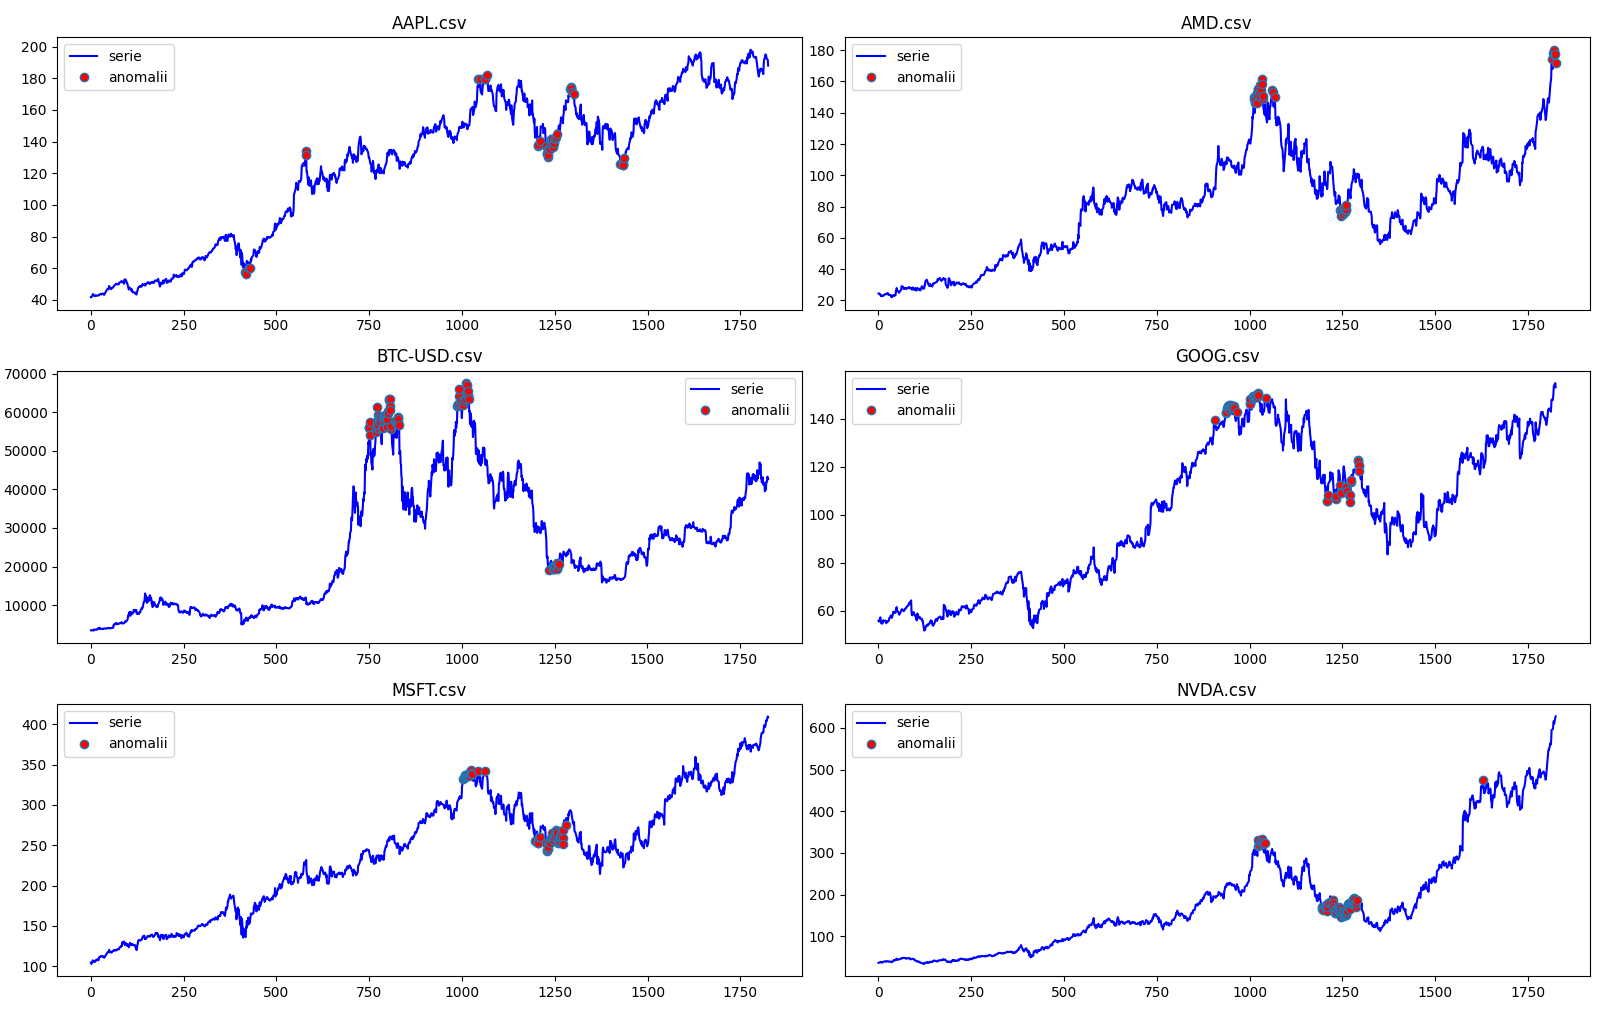
\includegraphics[width=\linewidth]{deviatie_absoluta.png}

%\chapter{Detectarea anomaliilor în ultimul punct al seriei}
%TBD
\chapter{Transformata Fourier pentru găsirea regiunilor cu anomalii}

\section{Scopul metodei}

Putem folosi această metodă pentru a găsi regiuni cu puncte anormale dintr-o serie de timp, anume regiuni în care punctele 
au caracteristici similare doar că foarte diferite faţă de vecinii lor din afara regiunii \cite{10.5555/1789574.1789615}.


Vom utiliza această idee doar pentru găsirea anomaliilor în date înregistrate în trecut, fapt ce ne-ar ajuta să analizăm 
impactul pe care anumite evenimente l-au avut asupra bursei de valori, precum o criză economică, şi astfel am putea prezice 
mai bine în viitor ce efect ar avea un eveniment similar. Metoda nu are ca scop prezicerea unor noi valori 
de pe bursă.

\section{Ideea din spatele metodei}

Transformata Fourier presupune că semnalul pe care îl analizează este \textbf{periodic} sau măcar foarte apropiat 
de unul periodic. Astfel, ar fi posibil să modelăm acest semnal folosind o sumă de sinusoide de frecvenţe diferite 
pentru seriile de timp complexe sau chiar cu o singură sinusoidă în cazul banal.

Aplicăm transformata Fourier pe seria de timp dată, iar apoi inversăm operaţia doar că vom păstra doar un număr $p$
de parametri, practic presupunâd ca \textbf{magnitudinea frecvenţelor} corespunzătoare este 0. Alegem să păstrăm doar primii 
$p$ parametri cu magnitudinile cele mai mari.

Apoi, folosind acest semnal, calculăm diferenţele între valorile eşantioanelor de pe aceeaşi poziţie(înregistrate la aceeaşi dată)
a ambelor semnale. Punctele care au o diferenţă absolută mai mare decât media diferenţelor absolute pentru toate punctele vor fi considerate
\textbf{potenţiale} anomalii. Pentru aceste potenţiale anomalii vom păstra într-un set $S$ diferenţa dintre valoarea seriei în punctul respectiv 
şi media a $c$ vecini ai săi de pe ambele părţi. Aplicăm \textbf{z-score} pentru fiecare punct din setul $S$, iar punctele a căror valoare 
depăşeşte un prag predefinit $t$ sunt considerate anomalii. Pentru găsirea regiunilor anormale, găsim 2 puncte consecutive cu z-score 
de \textbf{semn opus} care vor marca începutul regiunii, iar pentru a marca finalul, găsim 2 puncte consecutive cu z-score de semn opus, doar 
că în ordine inversă faţă de semnele care marchează începutul.

Punctele cu z-score pozitiv sunt asociate cu \textbf{vârfuri}, în timp ce cele cu semn negativ sunt asociate \textbf{văilor}. Din acest motiv,
acest algoritm funcţionează cel mai bine atunci când datele suferă schimbări \textbf{bruşte în frecvenţă}. Dacă schimbările se întâmplă gradual,
este posibil să nu mai găsim aceste diferenţe majore pentru z-score care să ne indice regiunile cu anomalii. Cu toate acestea, complexitatea 
de timp scăzută a algoritmului, anume $O(n \log n)$ datorită transformării Fourier rapide, face această metodă atractivă atunci când 
eficienţa este un criteriu important.

\section{Reprezentarea matematică}

\[ X[k] = \sum_{n=0}^{N-1} x[n] \cdot e^{-j\frac{2\pi}{N}kn} \]

\[ y[n] = \frac{1}{N} \sum_{k=0}^{N-1} X[k] \cdot e^{j\frac{2\pi}{N}kn} \] cu $X[k]=0$ dacă $k \notin P$, unde $P$ este setul parametrilor
cu cele mai mari $p$ magnitudini. $x$ este semnalul iniţial, $X$ este transformarea semnalului în domeniul frecvenţă, iar y este 
semnalul rezultat după trunchierea frecvenţelor.

\[ S = \{ x[i] - medie(vecini) | abs(x[i] - y[i]) > abs(medie(x - y))\} \] unde $vecini = \{x[j] | j \in [i - c, i + c], i \neq j \}$
\[ A = \{ i | abs(z[i]) > t \}\] unde $z = \{\frac{s[i] - mean(S)}{std(S)} | s \in S\}$ este z-score.

\section{Rezultate şi concluzii}

Pentru alegerea pragului $t$ vom folosi cuantila de 0.99 din vectorul de z-score calculat, întrucât presupunem ca numărul de 
anomalii este mult mai mic decât cel al punctelor normale.

Numărul de parametri $p$ îl menţinem mic, chiar sub 0.1\% din numărul total de parametri, deoarece seriile de timp de pe bursa 
de valori au o periodicitate aproape inexistentă şi astfel ar domina componenta medie doar că având foarte mult zgomot adăugat, 
deci practic am fi comparat semnalul iniţial aproape cu o linie orizontală.

Numărul $c$ de vecini influenţează probabilitatea ca un punct ce este potenţial anomalie să fie detectat ca anomalie după testul cu z-score.
Dacă includem mulţi vecini în media calculată, există o posibilitate mai mare de a include puncte ce deviază faţă de medie, deci un punct
ce ar fi avut o mică şansă să fie detectat ca anomalie, acum va fi acoperit de punctele ce deviază şi ele, micşorând diferenţa rezultată.
În cazul opus, dacă includem mai puţini vecini, iar aceştia diferă cu mult faţă de potenţiala anomalie, atunci va avea o şansă mai mare 
să treacă de testul z-score.

Mai există încă 2 parametri pe care îi numim $max_local$ şi $max_region$ care influenţează numărul maxim de puncte detectate ca
anomalii pe care suntem dispuşi să îi lăsăm între 2 anomalii cu z-score de semn opus, respectiv numărul maxim de puncte dintr-o regiune
cu anomalii. Primul parametru, intuitiv, reprezintă cât de mult vrem să lăsăm semnalul să crească sau să descrească gradual până se atinge 
o schimbare de semn, astfel, o valoare mai mică favorizează schimbările bruşte, pe când o valoare mai mare favorizează schimbările mai line.
Al doilea parametru, practic, ne arată care este lungimea maximă a unui "plafon" cu anomalii, anume până la o schimbare de semn a z-score.
În general, vom presupune că regiunile cu anomalii se întâmplă pe o perioadă scurtă de timp pentru că altfel nu ar mai fi considerate anomalii.

Mai jos se pot vedea rezultatele obţinute pentru 6 tipuri de acţiuni.

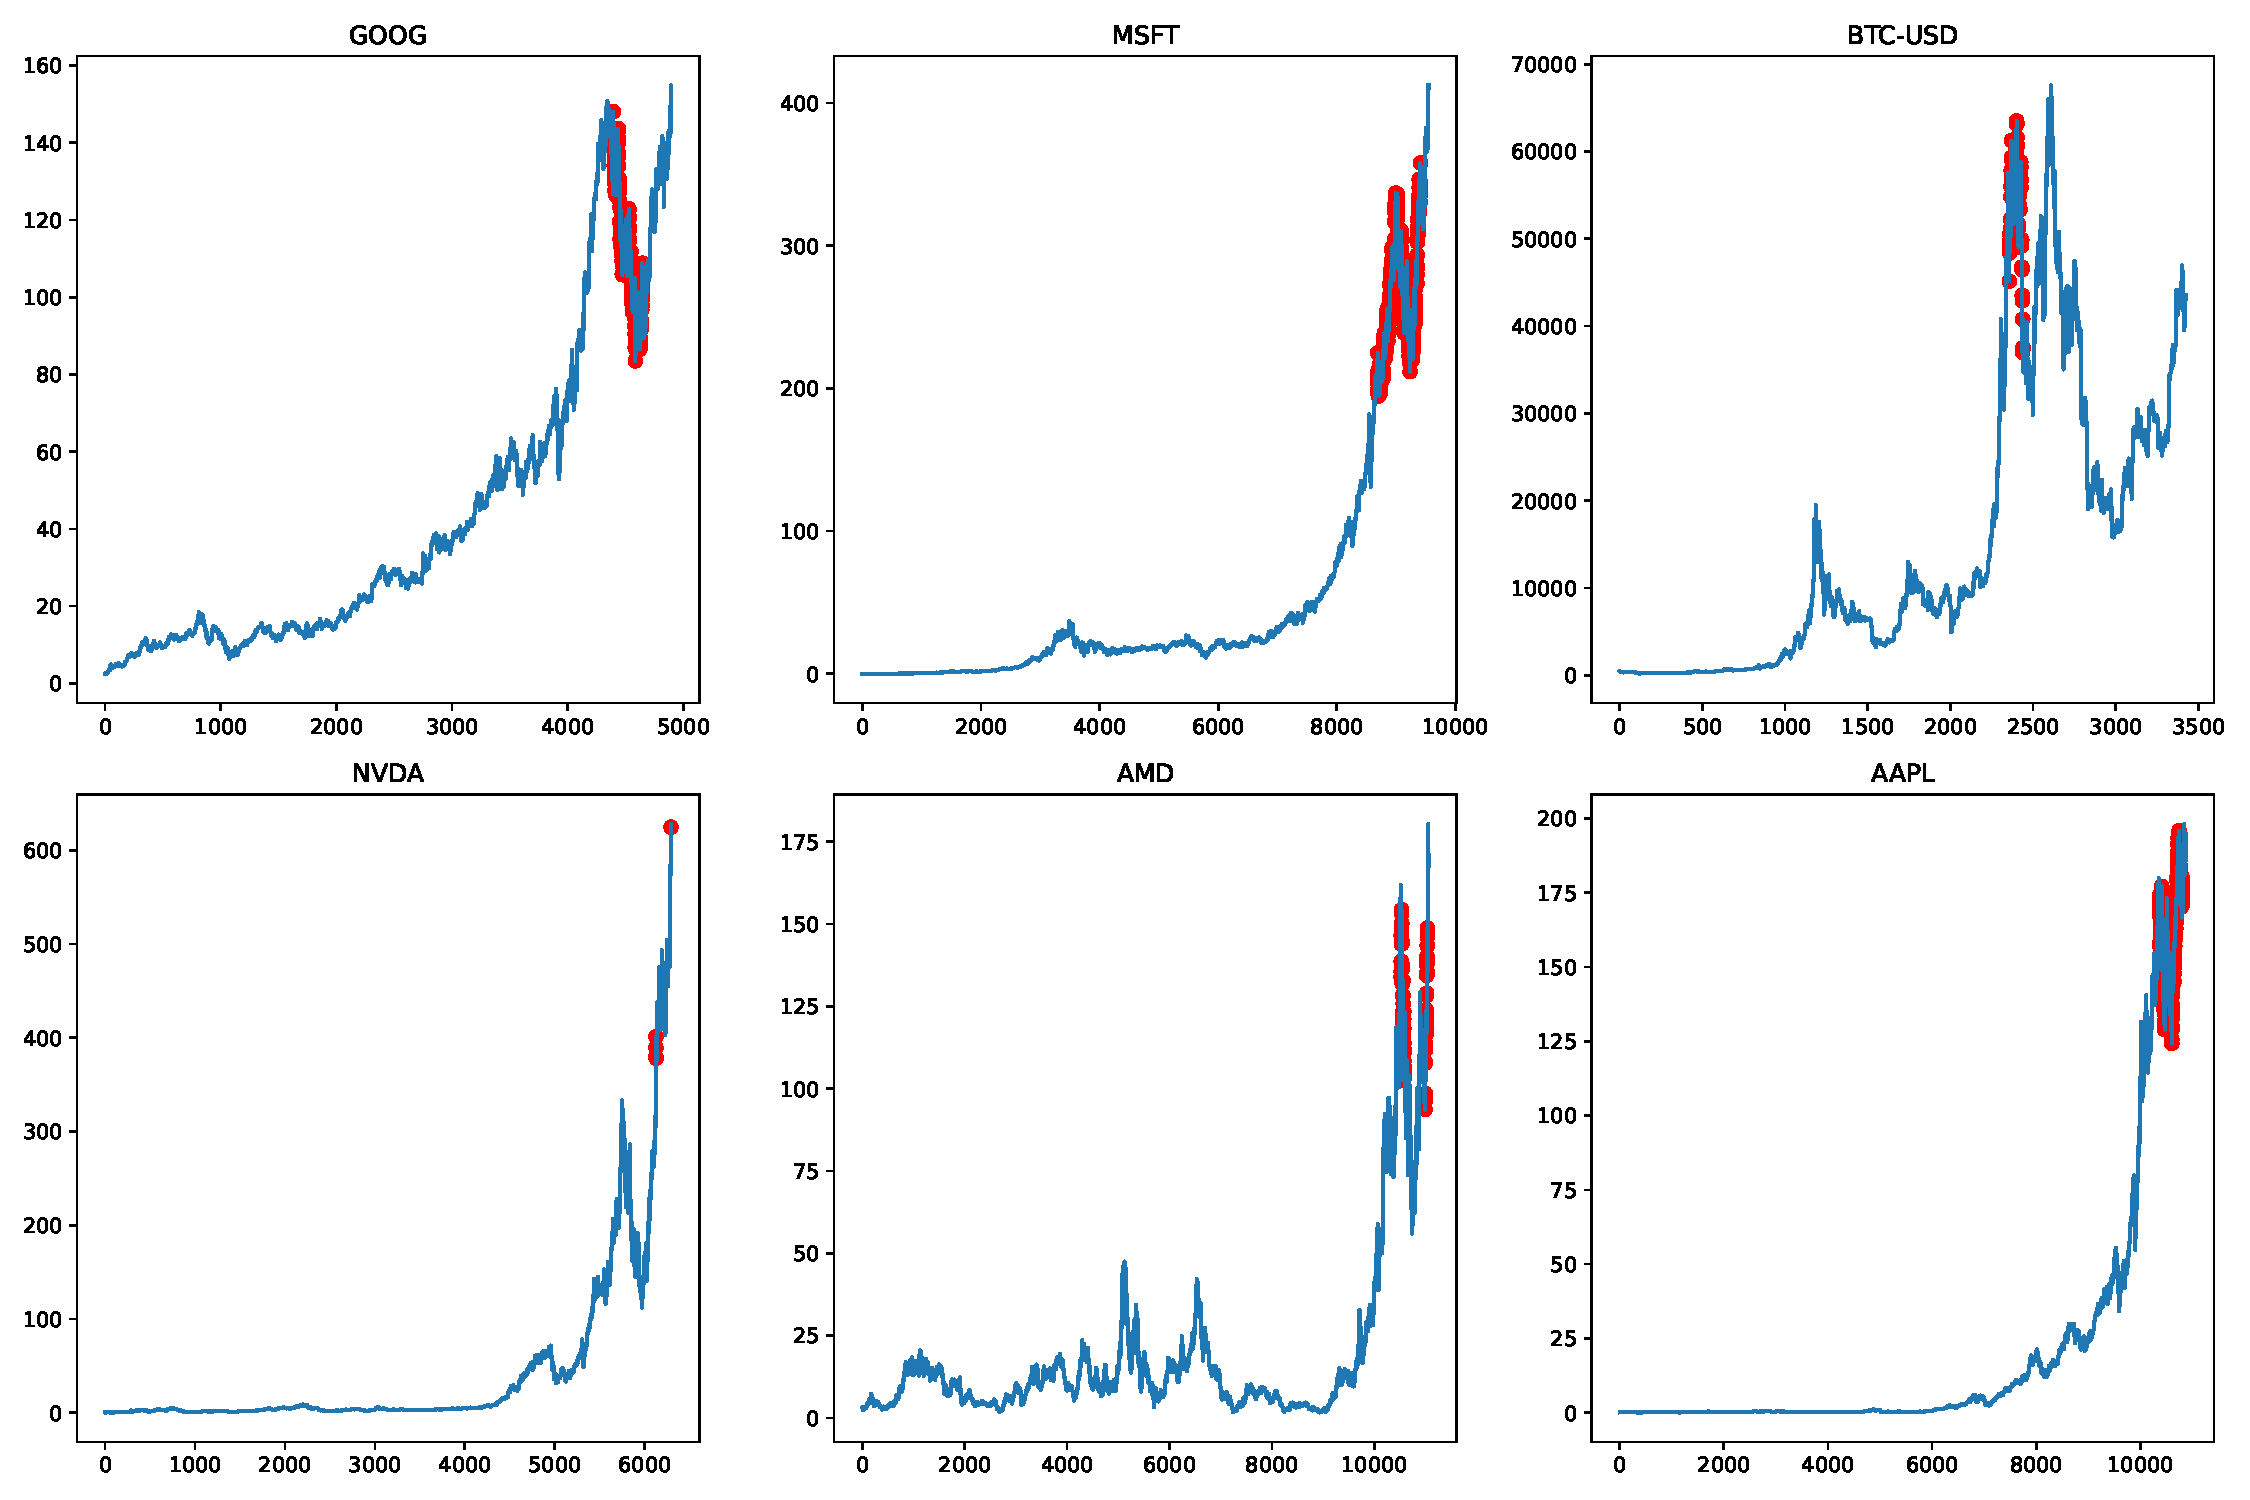
\includegraphics[width=\linewidth]{images/fft_results.pdf}
\chapter{Modelul ARMA}

\section{Scopul metodei}

Putem folosi această metodă pentru a prezice următoarele puncte dintr-o serie de timp, cu o acurateţe ce în mod natural va scădea
cu cât încercăm să vedem mai mult în viitor, şi astfel putem să semnalăm o posibilă anomalie dacă noul eşantion pe care credem că îl vom obţine şi în realitate, deviază cu mult faţă de punctele înregistrate deja.

Pentru a decide dacă un nou punct este sau nu anomalie, vom folosi un prag care este influenţat într-o proporţie majoră de volatilitatea instrumentului, anume indicatorul beta despre care am vorbit în 
introducere.

Acest model funcţionează bine atunci când datele din viitor pot fi modelate cu ajutorul datelor din trecut. Dacă nu există nicio relaţie între
evenimentele din trecut şi cele din viitor, atunci modelul nu va putea extrage caracteristicile necesare prezicerii.

\section{Ideea din spatele metodei}

Acest model este compus din 2 părţi, AR(AutoRegressive) şi MA(Moving-Average).

Partea autoregresivă încearcă sa modeleze punctele din seria de timp folosind o regresie liniară bazată pe un număr finit de puncte din trecut
la care se adaugă şi o variabilă de eroare care se poate presupune că este independent şi identic distribuită, provenită dintr-o distribuţie Gaussiană. Numărul de puncte din trecut este notat cu $p$ şi reprezintă singurul hiperparametru pentru această componentă.

Partea de medie glisantă încearcă să modeleze termenul eroare folosind o combinaţie liniară dintr-un număr de termeni de eroare din trecut. Despre aceste erori, putem face aceleaşi presupuneri ca mai sus. Numărul de termeni eroare din trecut este notat cu $q$ şi reprezintă
hiperparametrul pentru această componentă.

Aceste 2 componente sunt însumate pentru a obţine modelul final pe care îl vom putea folosi pentru a prezice noile puncte din seria de timp.

Găsirea hiperparamterilor optimi se poate realiza cu ajutorul funcţiei de autocorelaţie parţială pentru aflarea lui $p$, iar pentru $q$ putem folosi
functia de autocorelaţie. Apoi, pentru rezolvarea sistemului rezultat se poate folosi tehnica celor mai mici pătrate.

\section{Reprezentarea matematică}

ARMA(p, q):
\[
X_t = \varepsilon_t + \sum_{i=1}^{p} \phi_i X_{t-i} + \sum_{j=1}^{q} \theta_j \varepsilon_{t-j}
\]

AR(p):
\[
X_t = \varepsilon_t + \sum_{i=1}^{p} \phi_i X_{t-i} 
\]

MA(q):
\[
X_t = \mu + \varepsilon_t + \sum_{j=1}^{q} \theta_j \varepsilon_{t-j}
\]

unde $X_t$ este seria de timp, $\varepsilon_t$ este termenul eroare, $\mu$ este media semnalului $X_t$ pe care o presupunem 0 de obicei, iar 
$\phi_i$ şi $\theta_j$ sunt parametrii pentru regresia liniară a modelului AR, respectiv pentru combinaţia liniară a modelului MA.

\section{Implementare}

\noindent Metoda ARMA se implementează în python cu ajutorul funcției ARIMA din $statsmodels$. Ținând cont că ARMA(p,q) = ARIMA(order=(p,0,q)), se stabilește $p$ la o zecime din lungimea seriei de timp și un prag superior pentru $q$ ($qmax$, probabil 5 pentru că ARIMA rulează lent).\\
Se construiește modelul ARMA(p,q) pentru fiecare q de la 1 la $qmax$ și se prezice următoarea valoare a seriei. Media valorilor obținute reprezintă predicția.\\
Dacă modulul diferenței dintre valoarea reală a seriei și predicție depășeste un anumit prag, se consideră anomalie.\\
Pragul se stabilește în funcție de predicțiile obținute pentru fiecare valoare a lui q.\\
\\
\textbf{Aplicare pentru ultima valoare a seriei}\\
Modelul ARMA se construiește pentru toată seria înafară de ultima valoare sau pe ultimele $k$\% valori înafară de ultima. Se aplică pașii anteriori pentru ultima valoare a seriei.\\
\\
\textbf{Aplicare pe seria generală}\\
Pentru fiecare $start$ de la 2$p$ până la $n-1$ se aplică același algoritm ca la aplicarea pentru ultima valoare a seriei trunchiate până la $start$, cu diferența că pragul care indică anomeliile poate fi setat ulterior dacă se cunoaște dinainte procentul de anomalii din serie.\\
\textbf{Exemplu de rulare}\\
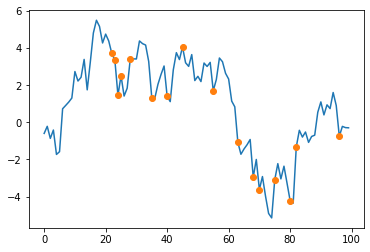
\includegraphics[width=\linewidth]{ARMA.png}
\chapter {Prophet}

\section {Despre Prophet}

\noindent Prophet \cite{prophet} este un model open-source dezvoltat de Facebook pentru analiza seriilor de timp, \^ in special pentru prognozare (``forecasting"). Aceast\u a libr\u arie separ\u a componentele de trend, sezoniere \c si reziduale, folosind \^ in spate regresie non-liniar\u a. Descompunerea seriei de timp se face \^ in felul urm\u ator: 

$$ y(t) = g(t) + s(t) + h(t) + \epsilon_t$$

unde $y$ este seria complet\u a de timp, $g$ este func\c tia de trend, $s$ este func\c tia de sezonalitate, $h$ este func\c tia care modeleaz\u a efectele vacan\c telor ce pot ap\u area \^ in mod neregulat asupra uneia sau mai multor zile, iar $\epsilon_t$ este termenul de eroare rezidual\u a \cite{prophet}. \\

%\noindent Prin arhitectura sa, acest model face prognoze analiz\^ and \^ intreaga serie de timp. Totu\c si, poate fi adaptat s\u a fac\u a detec\c tia unei anomalii doar \^ in ultimul punct, \^ intr-un mod care nu este foarte eficient, a\c sa cum este detaliat \^ in capitolul urm\u ator. \\

\section {Formatul predic\c tiilor}

\noindent Din punct de vedere al predic\c tiilor, pentru fiecare punct din prognoza generat\u a de Prophet, avem $3$ valori: \texttt{yhat}, \texttt{yhat\_lower} \c si \texttt{yhat\_upper}. Ultimele dou\u a valori reprezint\u a limitele intervalului de incertitudine, \^ in timp ce \texttt{yhat} este valoarea estimat\u a pe baza acestor valori. Pe baza datelor din trecut, am calculat o eroare absolut\u a (diferen\c ta dintre valoarea actual\u a si cea prezis\u a), respectiv un factor de incertitudine (diferen\c ta \^ intre capetele intervalului de incertitudine). Am considerat anomalii acele puncte pentru care eroarea era mai mare dec\^ at pragul de incertitudine, \^ inmul\c tit cu un factor setat. \\

\section {G\u asirea factorului optim, rezultate \c si concluzii}

\noindent Prima \^ incercare a fost aplicarea metodei procentuale pe Prophet, dar aceasta nu a mers pentru c\u a este func\c tional\u a doar dac\u a num\u arul de anomalii depinde monoton de un singur parametru. \^ In continuare, factorul a fost determinat din mai multe rul\u ari (\c si rezultatele cele mai bune au fost ob\c tinute pe intervalul $\interval{1.25}{1.5}$, i.e o eroare mai mare cu $25\%$ - $50\%$ dec\^ at intervalul de incertitudine). \\

\noindent Totodat\u a, pentru a stabili relevan\c ta rezultatelor ob\c tinute din aceste rul\u ari, am ales mai multe instrumente financiare, cu diverse volatilit\u a\c ti si sezonalit\u a\c ti, select\^ andu-le cu ajutorul indicatorului $\beta$. Am comparat rezultatele ob\c tinute de Prophet pentru detectarea de anomalii cu ajutorul a trei instrumente: Ethereum (este cunoscut faptul c\u a pe pia\c ta de criptomonede volatilitatea este mult mai mare), AAPL (o ac\c tiune cu volatilitate medie, av\^ and $\beta = 1.29$ la momentul redact\u arii) \c si VZ (o ac\c tiune cu volatilitate mic\u a, av\^ and $\beta = 0.38$ la momentul redact\u arii). Graficile prezentate arat\u a ultimii 5 ani din seriile de timp, dar Prophet a fost antrenat cu \^ intreg setul de date disponibil pe Yahoo Finance. \\

\noindent Din punct de vedere al m\u asur\u arii erorilor, modelul a ob\c tinut rezultate foarte bune, ob\c tin\^ and valoarea erorii mediii absolute procentuale \^ in jurul valorilor $0.1\%$ - $0.2\%$ \^ in cazul ac\c tiunilor \c si \^ in jur de $1\%$ pentru criptomonede. 

\begin{wrapfigure}[16]{r}{0.5\textwidth}
%\begin{center}
    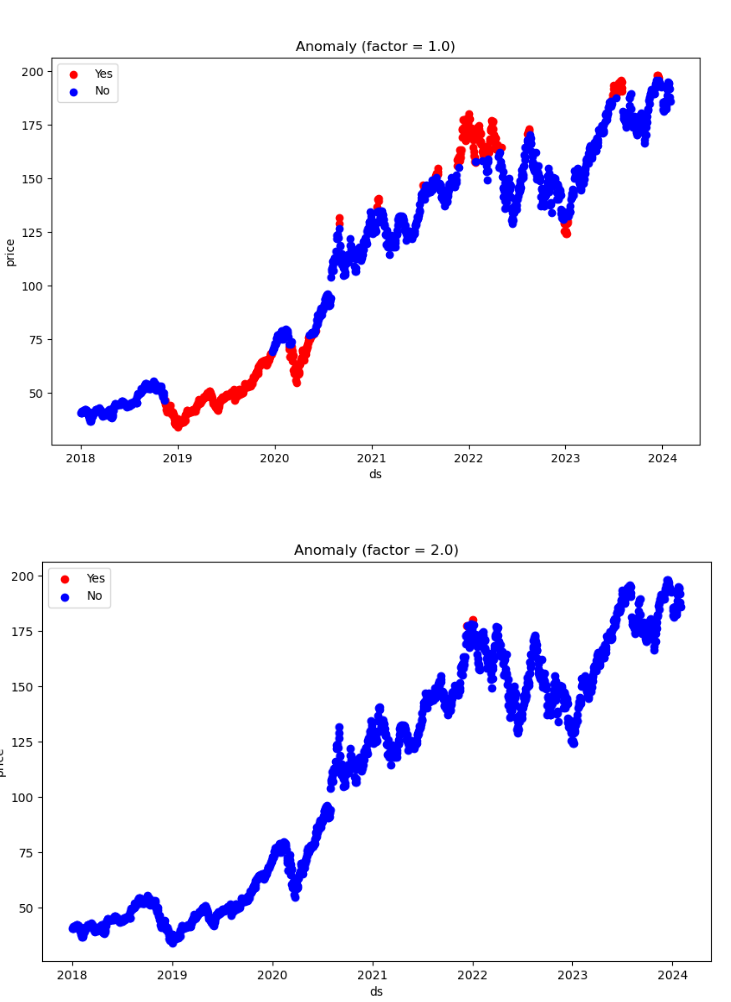
\includegraphics[width=0.48\textwidth]{apple_12.png}
  %\end{center}
\end{wrapfigure}

\hfill \break 

\noindent Am \^ inceput prin a selecta valorile $1$ \c si $2$ pentru factor pe ac\c tiunea AAPL, pentru a vedea cum se comport\u a modelul. \\ \\ A\c sa cum reiese din grafice, pentru valoarea $1$ a detectat multe valori ca anomalii, \^ in timp ce pentru valoarea $2$ a detectat una singur\u a, pe v\^ arful de la sf\^ ar\c situl anului 2021. Prin urmare, pentru a verifica dac\u a factorul $2$ este \^ intr-adev\u ar prea mare pentru ca modelul s\u a detecteze anomalii, am ales un instrument mult mai volatil, \c si anume ETH-USD (Ethereum).

\newpage 

\noindent Chiar \c si \^ in acest caz, detectarea anomaliilor este una redus\u a pentru un instrument at\^ at de volatil, a\c sa c\u a urm\u atoarul experiment a implicat rularea ambelor instrumente cu factorul $1.5$. 

\begin{wrapfigure}[16]{l}{0.5\textwidth}
%\begin{center}
    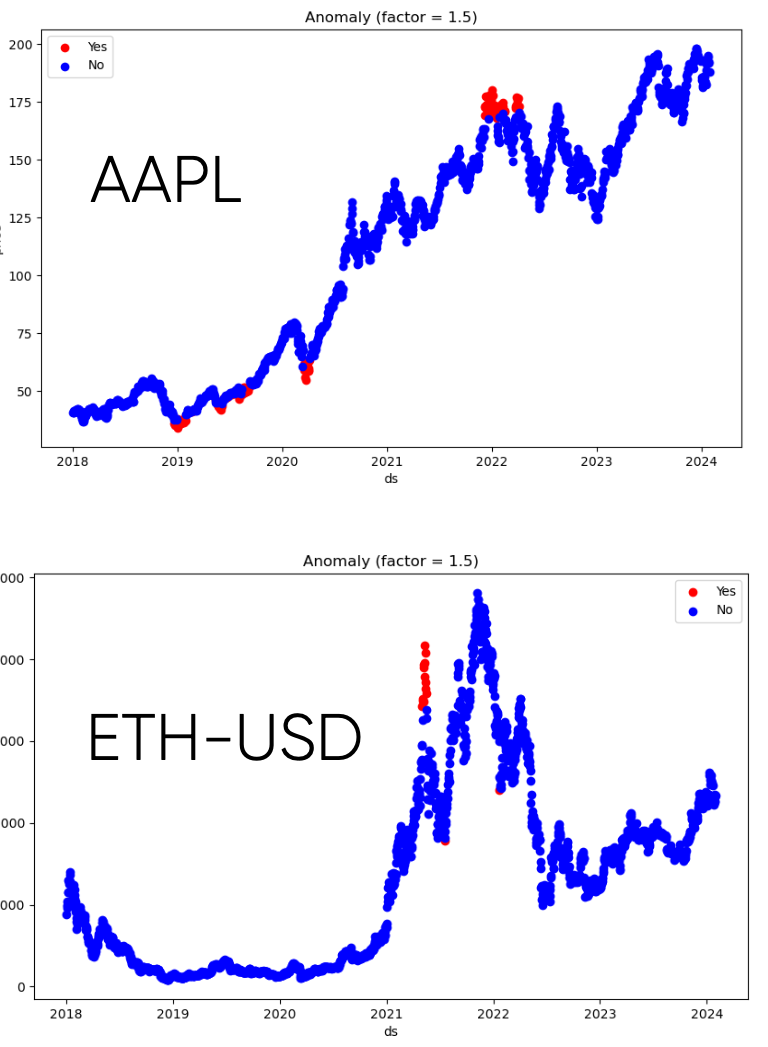
\includegraphics[width=0.48\textwidth]{15.png}
  %\end{center}
\end{wrapfigure}

\hfill \break

\noindent Se poate observa c\u a modelul \^ incepe s\u a dea rezultate de o calitate mai bun\u a, detect\^ and mai multe puncte de minim \c si mai multe de maxim (puncte ce sunt bune pentru efectuare de tranza\c tii de long, respectiv short, \^ in contextul unui program de trading algoritmic). \\
\noindent Aceast\u a valoare este una bun\u a, a\c sa c\u a urmeaz\u a s\u a fie validat\u a \c si pentru ac\c tiunea VZ. Totodat\u a, pentru a verifica dac\u a o valoare mai mic\u a poate ob\c tine rezultate mai bune, este nevoie de o rulare pe toate cele trei instrumentele folosite p\^ ana acum, cu valoarea factorului de $1.25$. 

\begin{wrapfigure}[5]{r}{0.5\textwidth}
%\begin{center}
    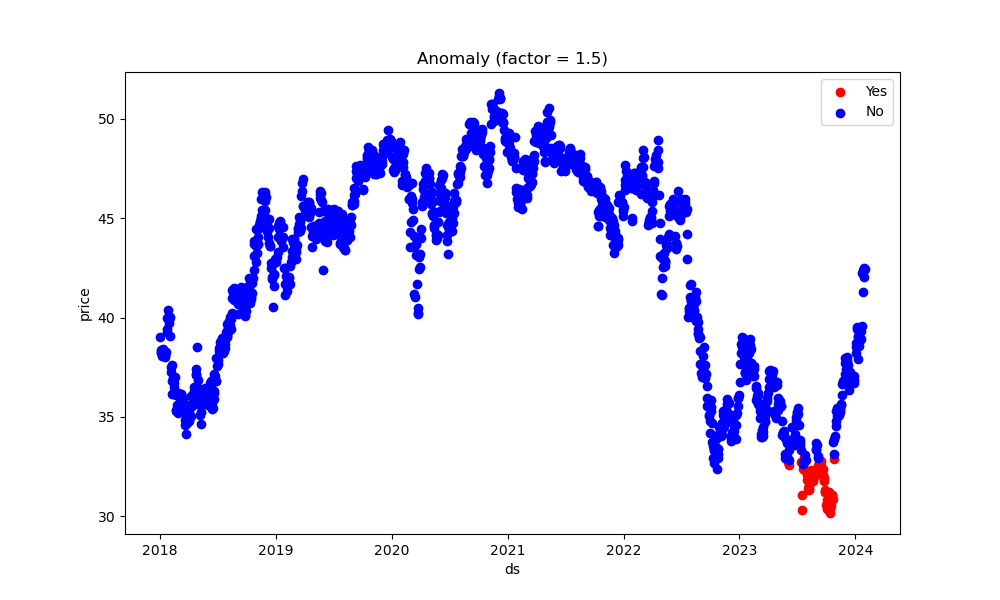
\includegraphics[width=0.48\textwidth]{VZ_1.5.png}
  %\end{center}
\end{wrapfigure}

\hfill \break 

\noindent Rezultatele ob\c tinute pentru VZ (imaginea din dreapta) confirm\u a faptul c\u a $1.5$ este un factor bun. Av\^ and $\beta$ mic, este de a\c steptat ca anomaliile detectate s\u a fie mai pu\c tine. 

\hfill \break 

\begin{center} 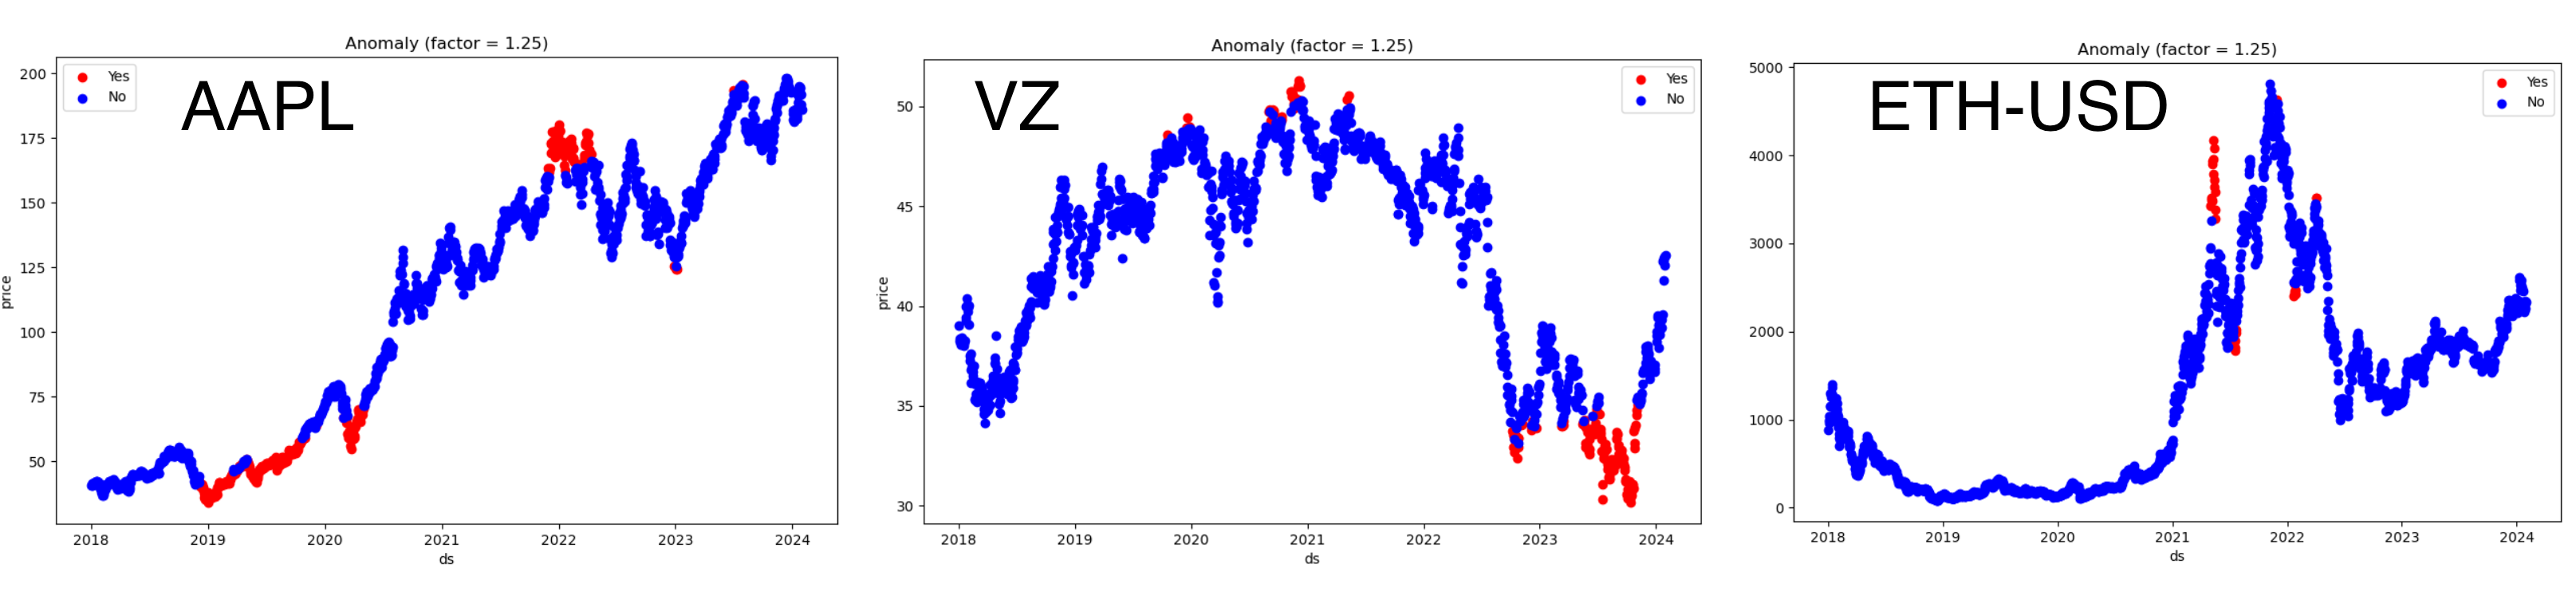
\includegraphics[width=\textwidth]{125.png} \end{center}

\noindent \c Si pentru factorul $1.25$ au fost ob\c tinute rezultate foarte bune, dar, \^ in mod evident, modelul este mai sensibil \c si va detecta mai multe anomalii. Prin urmare, \^ in functie de comportamentul a\c steptat de c\u atre utilizator, acest prag poate fi situat \^ intre $1.25$ \c si $1.5$. 

\printbibliography[heading=bibintoc]

\end{document}